%%----------------------------------------------------------------------------
%% Onderzoekstechnieken: Analyse van 2 kwantitatieve variabelen
%%----------------------------------------------------------------------------

\documentclass[aspectratio=169]{beamer}

%==============================================================================
% Aanloop
%==============================================================================

%---------- Vormgeving --------------------------------------------------------

\usetheme{hogent}

\usecolortheme{hgwhite} % witte achtergrond, zwarte tekst

\usepackage{graphicx,multicol}
\usepackage{comment,enumerate,hyperref}
\usepackage{amsmath,amsfonts,amssymb}
\usepackage[english]{babel}
\usepackage{multirow}
\usepackage{eurosym}
\usepackage{listings}
\usepackage{textcomp}
\usepackage{framed}
\usepackage{wrapfig}
\usepackage{tabu} %needed for \tabulinesep
\usepackage{wrapfig}
\usepackage{pgf-pie}
\usepackage{pgfplots}
\usepackage{booktabs}
\usepackage{pgfplotstable}
\usepackage{changepage}
\usepackage{ulem} % for \sout{text} (strikethrough)
\usepackage{fancyvrb} % for \begin{Verbatim} (LaTeX controls within verbatim)

%---------- Configuratie ------------------------------------------------------

\pgfplotsset{compat=1.16}
\usetikzlibrary{arrows,shapes,backgrounds,positioning,shadows}
\usetikzlibrary{pgfplots.statistics}

%---------- Commando-definities -----------------------------------------------

\newcommand{\tabitem}{~~\llap{\textbullet}~~}
\newcommand{\alertbox}[2][hgblue]{%
  \setbeamercolor{alertbox}{bg=#1,fg=white}
  \begin{beamercolorbox}[sep=2pt,center]{alertbox}
    \textbf{#2}
  \end{beamercolorbox}
}
\pgfmathdeclarefunction{gauss}{2}{%
  \pgfmathparse{1/(#2*sqrt(2*pi))*exp(-((x-#1)^2)/(2*#2^2))}%
}

%---------- Info over de presentatie ------------------------------------------

\title{Chapter 6. Bivariate Analysis: quantitative - quantitative}
\subtitle{Research Techniques}
\author{Jens Buysse \and Pieter-Jan Maenhaut \and Bert {Van Vreckem}}
\date{AY 2020-2021}

%==============================================================================
% Inhoud presentatie
%==============================================================================

\begin{document}

\begin{frame}
  \maketitle
\end{frame}

\begin{frame}
  \frametitle{What's on the menu?}
  
  \tableofcontents
\end{frame}

\begin{frame}
  \frametitle{Learning Goals}
  
  \begin{itemize}
    \item Regression analysis
    \item Covariance, correlation coefficient, coefficient of determination
  \end{itemize}
\end{frame}

\begin{frame}
  \frametitle{Overview}
    \centering
    \begin{tabular}{lll}
    	\toprule
    	\textbf{Independent}    & \textbf{Dependent}    & \textbf{Test/Metric}          \\
    	\midrule
      Qualitative             & Qualitative           & $\chi^2$-test                 \\
                              &                       & Cramér's $V$                  \\
      Qualitative             & Quantitative          & two-sample $t$-test           \\
    	                        &                       & Cohen's $d$                   \\
      Quantitative            & Quantitative          & ---                           \\
    	                        &                       & Regression, correlation       \\
    	\bottomrule
    \end{tabular}
\end{frame}

\section{Linear Regression}

\begin{frame}
  \frametitle{Linear Regression}
  \alertbox{With \textcolor{hgyellow}{regression} we will try to find a \textcolor{hgyellow}{consistent} and \textcolor{hgyellow}{systematic} relationship between the variables.}
  
  
  \begin{enumerate}
    \item \textbf{Monotonic:} general direction of the relationship between the two variables can be indicated (increasing/decreasing).
    \item \textbf{Non-monotonic:}  the presence (or absence) of one variable is systematically related to the presence (or absence) of another variable.
  \end{enumerate}
\end{frame}

\begin{frame}
  \frametitle{Linear Regression}
  Linear relationship: a linear relationship between an independent and dependent variable, where knowledge of the independent variable gives knowledge about the dependent variable.
  \begin{itemize}
    \item Presence: is there a relationship?
    \item Direction: increasing or decreasing?
    \item Strength of the relationship: strong, moderate, nonexistent, \dots
  \end{itemize}
\end{frame}

\begin{frame}
  \frametitle{Linear Regression}
  \centering
  \begin{tikzpicture}
  \begin{axis}[
  axis x line=middle,
  axis y line=middle,
  enlarge y limits=true,
  width=.9\textwidth, height=.9\textheight,     % size of the image
  grid = major,
  grid style={dashed, gray!30},
  ylabel=$y$,
  xlabel=$x$,
  legend style={at={(0.1,-0.1)}, anchor=north}
  ]
  \addplot[only marks] table  {data/regressie.dat};
  %\addplot [no markers, thick, red] table [y={create col/linear regression={y=y}}] {data/regressie.dat};
  \end{axis}
  \end{tikzpicture}
\end{frame}

\begin{frame}
  \frametitle{Linear Regression}
  \centering
  \begin{tikzpicture}
  \begin{axis}[
  axis x line=middle,
  axis y line=middle,
  enlarge y limits=true,
  width=.9\textwidth, height=.9\textheight,     % size of the image
  grid = major,
  grid style={dashed, gray!30},
  ylabel=$y$,
  xlabel=$x$,
  legend style={at={(0.1,-0.1)}, anchor=north}
  ]
  \addplot[only marks] table  {data/regressie.dat};
  \addplot [no markers, thick, red] table [y={create col/linear regression={y=y}}] {data/regressie.dat};
  \end{axis}
  \end{tikzpicture}
\end{frame}

\begin{frame}[plain]
  \frametitle{Method of least squares}
  \framesubtitle{Example}
  \begin{columns}
    \begin{column}{0.5\textwidth}
      
      \begin{figure}
        \centering
        
\includegraphics[height=.6\textheight]{les3-santa.png}
        \label{fig:les3-santa}
      \end{figure}
      
    \end{column}
    \begin{column}{0.5\textwidth}
      
      \begin{figure}
        \centering
        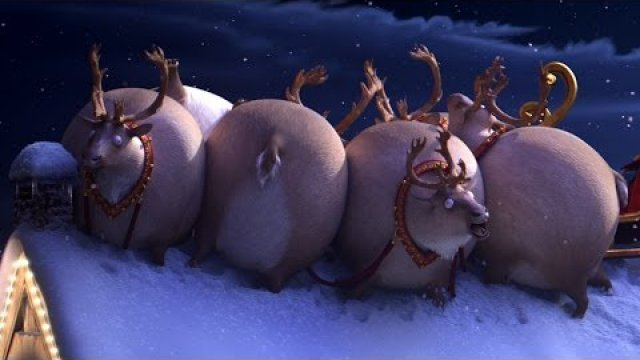
\includegraphics[width=1.00\textwidth]{les3-reindeer.jpg}
        \label{fig:les3-reindeer}
      \end{figure}
      
    \end{column}
  \end{columns}

  \bigskip
  Santa Claus wants to increase the weight of his reindeer. Is there a relationship between the protein content of the food and the weight gain of the reindeer?
  
\end{frame}

\begin{frame}
  \frametitle{Method of least squares}
  \framesubtitle{Example}
  
  \begin{table}[h]
    \centering
    \small
    \begin{tabular}{@{}rr@{}} \toprule
      Protein content\%& Weight gain (grams)  \\
      \midrule
      0   & 177 \\
      10  & 231 \\
      20  & 249 \\
      30  & 348 \\
      40  & 361 \\
      50  & 384 \\
      60  & 404 \\
      \bottomrule
    \end{tabular}
  \end{table}
\end{frame}

\begin{frame}
  \frametitle{Method of least squares}
  \framesubtitle{Example}
  
  \centering
  \begin{tikzpicture}
  \begin{axis}[
  axis x line=middle,
  axis y line=middle,
  enlarge y limits=true,
  width=.9\textwidth, height=.9\textheight,     % size of the image
  grid = major,
  grid style={dashed, gray!30},
  ylabel=weight gain (g),
  xlabel=protein content (\%),
  legend style={at={(0.1,-0.1)}, anchor=north}
  ]
  \addplot[only marks] table  {data/santa.txt};
  % \addplot [no markers, thick, red] table [y={create col/linear regression={y=y}}] {data/santa.txt};
  \end{axis}
  \end{tikzpicture}
\end{frame}

\begin{frame}
  \frametitle{Method of least squares}
  \framesubtitle{Example}
  
  \begin{table}[h] \centering \footnotesize
    \begin{tabular}{@{}llllll@{}}
      \toprule
      $x$   & $y$     & $x-\overline{x}$    & $y - \overline{y}$        & $(x-\overline{x})(y - \overline{y})$       &  $(x-\overline{x})^{2}$    \\ \midrule
      0  & 177 & -30 & -130,71 & 3921,3 & 900  \\
      10 & 231 & -20 & -76,71  & 1534,2 & 400  \\
      20 & 249 & -10 & -58,71  & 587,1  & 100  \\
      30 & 348 & 0   & 40,29   & 0      & 0    \\
      40 & 361 & 10  & 53,29   & 532,9  & 100  \\
      50 & 384 & 20  & 76,29   & 1525,8 & 400  \\
      60 & 404 & 30  & 96,29   & 2888,7 & 900  \\
      &     &     &         & 10990  & 2800 \\ \bottomrule
    \end{tabular}
    \caption{Calculations required to apply the method of least squares.}
    \label{tab:rendieren2}
  \end{table}
\end{frame}

\begin{frame}
  \frametitle{Method of least squares}
  \framesubtitle{Equation}
  
  The regression line has the following equation:
  
  \[ \hat{y} = \beta_1 x + \beta_0 \]
  
  with:
  
  \[ \beta_{1} = \frac{\sum_{i=1}^{n} (x_{i}-\overline{x})(y_{i} - \overline{y})}{\sum_{i=1}^{n} (x-\overline{x})^{2}} = \frac{10990}{2800} = 3.925 \]
  \[ \beta_{0} = \overline{y} - \beta_{1} \overline{x} = 307.7143 - 3.925 \times 30 = 189.96 \]
  
  Note: $\hat{y}$ indicates ``an estimation for $y$''
\end{frame}

\begin{frame}
  \frametitle{Method of least squares}
  \framesubtitle{Example}
  
  \centering
  \begin{tikzpicture}
  \begin{axis}[
  axis x line=middle,
  axis y line=middle,
  enlarge y limits=true,
  width=.9\textwidth, height=.9\textheight,     % size of the image
  grid = major,
  grid style={dashed, gray!30},
  ylabel=weight gain (g),
  xlabel=protein content (\%),
  legend style={at={(0.1,-0.1)}, anchor=north}
  ]
  \addplot[only marks] table  {data/santa.txt};
  \addplot [no markers, thick, red] table [y={create col/linear regression={y=y}}] {data/santa.txt};
  \end{axis}
  \end{tikzpicture}
\end{frame}

\section{Correlation coefficient and Coefficient of determination}

\begin{frame}
  \frametitle{Covariance}
  
  \alertbox{Covariance is a measure that indicates whether a relationship between two variables is increasing or decreasing.}
  
  \[ \mathrm{Cov}(X, Y) = \frac{1}{n-1} \sum_{i = 1}^{n} (x_i - \overline{x}) (y_i - \overline{y}) \]
  
  $\mathrm{Cov} > 0$: increasing
  
  $\mathrm{Cov} \approx 0$: no relationship
  
  $\mathrm{Cov} < 0$: decreasing

  \strong{Note} Covariance of population (denominator $n$) vs. sample (denominator $n-1$)
\end{frame}

\begin{frame}
  \frametitle{Covariance}
  Family size of 15 families compared to the family size of the mother.
  
  \centering
  \begin{tikzpicture}
  \begin{axis}[
  axis x line=middle,
  axis y line=middle,
  enlarge y limits=true,
  width=.9\textwidth, height=.9\textheight,     % size of the image
  grid = major,
  grid style={dashed, gray!30},
  ylabel=family size mother,
  xlabel=family size,
  legend style={at={(0.1,-0.1)}, anchor=north}
  ]
  \addplot[only marks] table  {data/families.txt};
  \addplot [no markers, thick, red] table [y={create col/linear regression={y=y}}] {data/families.txt};
  \end{axis}
  \end{tikzpicture}
  
  We have that $\overline{x} = 3$ and $\overline{y} = 4.3$.
\end{frame}

\tikzset{small dot/.style={fill=black, circle,scale=0.2}}
\tikzset{every pin/.style={draw=black,fill=yellow!10}}

\begin{frame}[plain]
  \frametitle{Covariance for linear relationship}
  \centering
  \begin{tikzpicture}
  \begin{axis}[
  axis x line=middle,
  axis y line=middle,
  enlarge y limits=true,
  width=.9\textwidth, height=.9\textheight,     % size of the image
  grid = major,
  grid style={dashed, gray!30},
  ylabel=family size mother,
  xlabel=family size,
  legend style={at={(0.1,-0.1)}, anchor=north}
  ]
  \draw (axis cs:3,0)--(axis cs:3,8);
  \draw (axis cs:0,4.3)--(axis cs:6,4.3);
  \node[small dot, pin=120:{$III$}] at (axis cs:1.9,6) {};
  \node[small dot, pin=120:{$I$}] at (axis cs:4.5,6) {};
  \node[small dot, pin=120:{$II$}] at (axis cs:1.9,2) {};
  \node[small dot, pin=120:{$IV$}] at (axis cs:4.5,2) {};
  \addplot[only marks] table  {data/families.txt};
  \end{axis}
  \end{tikzpicture}
\end{frame}

\begin{frame}[plain]
  \frametitle{Covariance for random variables}
  \centering
  \footnotesize
  \begin{tikzpicture}
  \begin{axis}[
  axis x line=middle,
  axis y line=middle,
  enlarge y limits=true,
  width=.9\textwidth, height=.9\textheight,     % size of the image
  grid = major,
  grid style={dashed, gray!30},
  ylabel=family size mother,
  xlabel=date of birth mother,
  legend style={at={(0.1,-0.1)}, anchor=north}
  ]
  \draw (axis cs:1942.625,0)--(axis cs:1942.625,6);
  \draw (axis cs:1930,3.4375)--(axis cs:1955,3.4375);
  \node[small dot, pin=120:{$III$}] at (axis cs:1935,5) {};
  \node[small dot, pin=120:{$I$}] at (axis cs:1950,5) {};
  \node[small dot, pin=120:{$II$}] at (axis cs:1935,2) {};
  \node[small dot, pin=120:{$IV$}] at (axis cs:1950,2) {};
  \addplot[only marks] table  {data/families2.txt};
  \end{axis}
  \end{tikzpicture}
  
  We have that $\overline{x} = 1942.625$ and $\overline{y} = 3.4375$.
\end{frame}

\begin{frame}
  \frametitle{Pearson correlation coefficient}
  
  \alertbox{The \textcolor{hgyellow}{Pearson correlation coefficient} $R$ is a measure for the strength of a linear correlation between $x$ and $y$}
  
  \begin{align}
  R & = \frac{Cov(X, Y)}{\sigma_{x} \sigma_{y}} \\
  & = \frac{\sum_{i = 1}^{n} (x_i - \overline{x}) (y_i - \overline{y})}
  {\sqrt{\sum_{i = 1}^n (x_i - \overline{x})^2}
    \sqrt{\sum_{i = 1}^n (y_i - \overline{y})^2}}
  \end{align}
  
  \[ R \in [-1, +1] \]
  
\end{frame}


\begin{frame}
  \frametitle{Interpretation correlation coefficient}
  
  \centering
  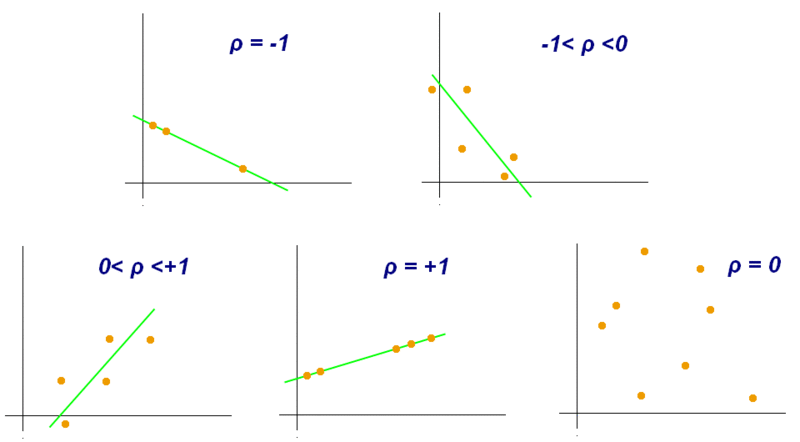
\includegraphics[height=.8\textheight]{les3-regressie.png}
  
\end{frame}

\begin{frame}
  \frametitle{Coefficient of determination}
  \alertbox{The \textcolor{hgyellow}{coefficient of determination} $R^2$ explains the percentage of the variance of the observed values relative to the regression line.}
  
  $R^2$: percentage variance observations explained by the regression line
  
  $1 - R^2$: percentage variance observations \textit{not} explained by regression
  
\end{frame}

\begin{frame}[plain]
  \frametitle{Coefficient of determination}
  \begin{figure}
    \resizebox{.7\textwidth}{.7\textheight}{
      \begin{tikzpicture}
        \begin{axis}[
        axis x line=middle,
        axis y line=middle,
        enlarge y limits=true,
        width=.9\textwidth, height=.9\textheight,     % size of the image
        grid = major,
        grid style={dashed, gray!30},
        ylabel=weight gain (g),
        xlabel=protein content (\%),
        legend style={at={(0.1,-0.1)}, anchor=north}
        ]
        \addplot[only marks] table  {data/santa.txt};
        \addplot [no markers, thick, red] table [y={create col/linear regression={y=y}}] {data/santa.txt};
        \addplot [mark=none, color=red] coordinates {
          (0,177) (0,189.9643)
        };
        \addplot [mark=none, color=red] coordinates {
          (10,231) (10,229.2143)
        };
        \addplot [mark=none, color=red] coordinates {
          (20,249) (20,268.4643)
        };
        \addplot [mark=none, color=red] coordinates {
          (30,348) (30,307.7143)
        };
        \addplot [mark=none, color=red] coordinates {
          (40,361) (40,346.9643)
        };
        \addplot [mark=none, color=red] coordinates {
          (50,384) (50,386.2143)
        };
        \addplot [mark=none, color=red] coordinates {
          (60,404) (60,425.4643)
        };
        
        \end{axis}
      \end{tikzpicture}
    }
    \label{fig:rendierenFiguur2}
    \caption{Deviations from the regression line: assumption that $x$ provides additional information for predicting $y$.}
  \end{figure}
\end{frame}

\begin{frame}[plain]
  \begin{figure}
    \resizebox{.7\textwidth}{.7\textheight}{
      \begin{tikzpicture}
        \begin{axis}[
        axis x line=middle,
        axis y line=middle,
        enlarge y limits=true,
        width=.9\textwidth, height=.9\textheight,     % size of the image
        grid = major,
        grid style={dashed, gray!30},
        ylabel=weight gain (g),
        xlabel=protein content (\%),
        ]
        \addplot[only marks] table  {data/santa.txt};
        \addplot [mark=none, color=black] coordinates {
          (0,307.71) (60,307.71)
        };
        \addplot [mark=none, color=red] coordinates {
          (0,177) (0,307.71)
        };
        \addplot [mark=none, color=red] coordinates {
          (10,231) (10,307.71)
        };
        \addplot [mark=none, color=red] coordinates {
          (20,249) (20,307.71)
        };
        \addplot [mark=none, color=red] coordinates {
          (30,348) (30,307.71)
        };
        \addplot [mark=none, color=red] coordinates {
          (40,361) (40,307.71)
        };
        \addplot [mark=none, color=red] coordinates {
          (50,384) (50,307.71)
        };
        \addplot [mark=none, color=red] coordinates {
          (60,404) (60,307.71)
        };
        
        \end{axis}
      \end{tikzpicture}
    }
    \label{fig:rendierenFiguur3}
    \caption{Deviations from the mean of y: assumption that $x$ provides no information for predicting $y$ ($\overline{y} =307.71$).}
  \end{figure}
\end{frame}

\begin{frame}
  \frametitle{Correlation coefficient and coefficient of determination}
  \centering
  \begin{table} \small
    \begin{tabular}{@{}rrrr@{}} \toprule
      $|R|$ & $R^{2}$ & Explained variance &  Interpretation \\
      \midrule
      $< 0.3$       & $< 0.1$       & $< 10\%$    & very weak \\
      $0.3 - 0.5$   & $0.1 - 0.25$ & $10 - 25\%$  & weak \\
      $0.5 - 0.7$   & $0.25 - 0.5$  & $25 - 50\%$ & moderate \\
      $0.7 - 0.85$  & $0.5 - 0.75$  & $50 - 75\%$ & strong\\
      $0.85 - 0.95$ & $0.75 - 0.9$  & $75 - 90\%$ & very strong\\
      $> 0.95$      & $> 0.9$       & $>90\%$     & exceptional(!)\\
      \bottomrule
    \end{tabular}
  \end{table}
  
\end{frame}

\begin{frame}
  \frametitle{Strength of relationship reindeer}
  \begin{columns}
    \begin{column}{0.5\textwidth}
      \begin{table}[h] \centering \small
        \begin{tabular}{@{}rrr@{}} \toprule
          $(x-\overline{x})$ & $(y - \overline{y})$ & $(x-\overline{x})(y - \overline{y})$ \\
          \midrule
          $-30$ & $-130.714$ & $3921.429$ \\
          $-20$ & $-76.7143$ & $1534.286$ \\
          $-10$ & $-58.7143$ & $587.1429$\\
          $0$   & $40.28571$ & $0$\\
          $10$  & $53.28571$ & $532.8571$\\
          $20$  & $76.28571$ & $1525.714$\\
          $30$  & $96.28571$ & $2888.571$\\
          \bottomrule
        \end{tabular}
      \end{table}
    \end{column}
    \begin{column}{0.5\textwidth}
      \[ \sum_{i}^{n} (x-\overline{x})(y - \overline{y}) = 10990 \]
      \[ Cov = \frac{10990}{7} = 1570 \]
      \[ \sigma_{x} = 20 \]
      \[ \sigma_{y} = 81.03 \]
      \[ R = \frac{1570}{20 \times 81.03} = 0.96 \]
      \[ R^{2} = 0.93 \]
    \end{column}
  \end{columns}
\end{frame}

\begin{frame}
  \frametitle{Considerations}
  \begin{itemize}
    \item The correlation coefficient only looks at the relationship between two variables. Interactions with other variables are not considered.
    \item The correlation coefficient explicitly does not assume a cause and effect relationship.
    \item The Pearson product-moment correlation coefficient only expresses linear relationships.
  \end{itemize}
\end{frame}

\end{document}